%%%%%%%% ICML 2023 REPORT: MOVIELENS-32M RECOMMENDER SYSTEM %%%%%%%%%%%%

\documentclass{article}

\usepackage{microtype}
\usepackage{graphicx}
\usepackage{subfigure}
\usepackage{booktabs}
\usepackage{hyperref}

\newcommand{\theHalgorithm}{\arabic{algorithm}}

\usepackage[accepted]{icml2023}

\usepackage{amsmath}
\usepackage{amssymb}
\usepackage{mathtools}
\usepackage{amsthm}
\usepackage[capitalize,noabbrev]{cleveref}

\theoremstyle{plain}
\newtheorem{theorem}{Theorem}[section]
\newtheorem{proposition}[theorem]{Proposition}
\newtheorem{lemma}[theorem]{Lemma}
\newtheorem{corollary}[theorem]{Corollary}
\theoremstyle{definition}
\newtheorem{definition}[theorem]{Definition}
\newtheorem{assumption}[theorem]{Assumption}
\newtheorem{remark}[theorem]{Remark}

\icmltitlerunning{Matrix Factorization and Genre-Based Recommender Systems on MovieLens-32M}

\begin{document}

\twocolumn[
\icmltitle{Matrix Factorization and Genre-Based Recommender Systems on MovieLens-32M}

\begin{icmlauthorlist}
\icmlauthor{Joel Gedeon Asa Mapa}{aims}
\end{icmlauthorlist}

\icmlaffiliation{aims}{African Institute for Mathematical Sciences (AIMS) South Africa, 6 Melrose Road, Muizenberg 7975, Cape Town, South Africa}
\icmlcorrespondingauthor{Joel Gedeon Asa Mapa}{joel@aims.ac.za}

\icmlkeywords{Recommender Systems, Matrix Factorization, Alternating Least Squares, MovieLens 32M, Cold-Start Recommendation}

\vskip 0.3in
]

\printAffiliationsAndNotice{}

\begin{abstract}
Building a recommender system for tens of millions of ratings requires both a solid statistical model and fast data structures. In this paper, we build and study matrix factorization models trained with Alternating Least Squares (ALS) on the full MovieLens-32M dataset ($32{,}000{,}204$ ratings from $200{,}948$ users and $84{,}432$ movies), as well as a smaller $5$-million-rating subset. To store the ratings efficiently in memory, we use two Compressed Sparse Row (CSR) matrices: one indexed by user and one indexed by movie. This setup uses about $513$~MB of RAM and allows us to look up all ratings for any user or movie in constant time. By parallelizing the ALS updates across CPU threads and solving the small linear systems in-place with Cholesky decomposition, our training loop runs nearly $70$ times faster than batched array solvers. We begin by exploring the rating distribution and power-law behavior of users and movies. Next, we compare a simple bias-only model against full matrix factorization with user and movie trait vectors, showing how regularization and the number of latent dimensions $K$ affect test error and overfitting. We also visualize 2D movie embeddings, generate personalized recommendations for a new user who likes \emph{The Lord of the Rings}, and identify the most and least polarizing movies using vector lengths. Finally, we extend the model by adding movie genre information into the prior distribution of movie vectors, which noticeably improves predictions for new and rarely rated movies. Our source code is publicly available at \url{https://github.com/joelinator/movielens-32m-recommender}.
\end{abstract}

\section{Introduction}
\label{sec:introduction}

Online platforms such as streaming services and online stores rely on recommender systems to help users find items they might enjoy among tens of thousands of choices \cite{koren2009matrix,harper2015movielens}. One of the most effective approaches to this problem is collaborative filtering, which predicts what a user will like based on past ratings from many users, without needing detailed descriptions of the items themselves.

When working with large datasets like MovieLens-32M, which has over $32$ million ratings across $200{,}948$ users and $84{,}432$ movies, storing the ratings in a standard two-dimensional table is not practical. A full table of size $200{,}948 \times 84{,}432$ using 32-bit floats would take $67.8$~GB of memory, even though $99.81\%$ of the entries are empty because most users only rate a small fraction of the catalog.

Matrix factorization handles this sparsity by representing each user $m$ and each movie $n$ with a short vector of $K$ numbers, $u_m \in \mathbb{R}^K$ and $v_n \in \mathbb{R}^K$, called latent trait vectors \cite{mnih2007probabilistic,koren2009matrix}. A rating is then predicted as the dot product $u_m^\top v_n$ plus baseline user and movie biases. To learn these parameters from observed ratings, two main algorithms are commonly used: Stochastic Gradient Descent (SGD) and Alternating Least Squares (ALS) \cite{zhou2008large}. ALS is especially attractive for large datasets for three reasons:
\begin{enumerate}
    \item It does not require tuning a learning rate, because each update step has an exact closed-form formula.
    \item The regularized loss function is guaranteed to decrease (or stay the same) at every single step.
    \item When all movie vectors are held fixed, each user vector can be updated independently of all other users. Likewise, when user vectors are fixed, all movie vectors can be updated in parallel across CPU cores.
\end{enumerate}

\subsection{Problem Statement and Structure of the Paper}

Our goal is to predict unseen movie ratings accurately at scale while also understanding what the model learns and where it struggles. Following a clear separation between data exploration, modeling, and experimental evaluation, the rest of this paper is organized as follows:
\begin{enumerate}
    \item \textbf{Data Representation and Exploration (\cref{sec:data_topology}):} We show how to store $32$ million ratings compactly in two CSR matrices ($\mathcal{S}_{\text{user}}$ and $\mathcal{S}_{\text{movie}}$) so that both user updates and movie updates run in constant lookup time, and we analyze the rating histogram and user/movie power-law distributions.
    \item \textbf{Models and ALS Optimization (\cref{sec:bias_model}):} We formulate all three of our models and derive their Alternating Least Squares (ALS) update steps in one place: (i) the baseline bias-only model (\cref{sec:bias_model_sub}), (ii) the matrix factorization model with user and movie trait vectors $U$ and $V$ (\cref{sec:latent_als}), and (iii) the genre-regularized matrix factorization model with altered loss function and three-step ALS updates (\cref{sec:genre_model}), together with our parallel in-place Cholesky solver (\cref{sec:fast_cholesky}).
    \item \textbf{Experimental Results (\cref{sec:experiments}):} We present a comprehensive evaluation across both MovieLens-5M and the full MovieLens-32M dataset, including our train/test split, bias-only and matrix factorization RMSE and monotonic loss curves, choice of training iterations, hyperparameter tuning ($\lambda, \gamma, \tau$), choice of best latent dimension $K$ and diminishing returns, runtime speedups on all $32$ million ratings, 2D movie and genre embeddings, \emph{Lord of the Rings} dummy-user recommendations, and most/least polarizing movies.
\end{enumerate}

\section{Data Representation and Exploratory Analysis}
\label{sec:data_topology}

\subsection{Dual Sparse Matrix Structure}
Let $M$ be the number of users and $N$ be the number of movies. The dataset consists of observed ratings $r_{m,n} \in \{0.5, 1.0, \dots, 5.0\}$ for user--movie pairs $(m,n) \in \Omega$, where $\Omega$ is the set of all observed interactions. For each user $m$, we write $\Omega_m = \{n : (m,n) \in \Omega\}$ for the set of movies rated by user $m$. Similarly, for each movie $n$, we write $\Omega^n = \{m : (m,n) \in \Omega\}$ for the set of users who rated movie $n$. The total number of ratings is $|\Omega| = \sum_{m=1}^M |\Omega_m| = \sum_{n=1}^N |\Omega^n|$.

During ALS training, updating user parameters requires looping over all movies rated by each user ($\Omega_m$), while updating movie parameters requires looping over all users who rated each movie ($\Omega^n$). If we only stored the data grouped by user, updating the movies would require either scanning the entire dataset repeatedly or jumping randomly in memory. Using Python lists of lists or dictionaries also uses too much memory and slows down CPU loops.

To make both half-steps fast, we store the ratings in two Compressed Sparse Row (CSR) structures:
\begin{itemize}
    \item \textbf{User-Indexed CSR Matrix ($\mathcal{S}_{\text{user}}$):} Uses three flat arrays: an offset array $p^{(u)}$ of length $M+1$, a movie-index array of length $|\Omega|$, and a rating array of length $|\Omega|$. For any user $m$, their rated movie IDs and ratings sit side-by-side in memory between indices $p^{(u)}_m$ and $p^{(u)}_{m+1}$.
    \item \textbf{Movie-Indexed CSR Matrix ($\mathcal{S}_{\text{movie}}$):} Uses the same layout transposed by movie: an offset array $p^{(v)}$ of length $N+1$, a user-index array of length $|\Omega|$, and a rating array of length $|\Omega|$. For any movie $n$, all users who rated it sit contiguously between indices $p^{(v)}_n$ and $p^{(v)}_{n+1}$.
\end{itemize}
Using 32-bit integers for indices and offsets and 32-bit floats for ratings, storing both CSR views takes $16|\Omega| + 4(M+N+2)$ bytes. As shown in \cref{tab:dataset_summary}, for all $32{,}000{,}204$ ratings in MovieLens-32M, both structures together take only $513.1$~MB of RAM (over $130$ times smaller than a dense matrix) and load from disk in $4.23$~seconds. Because the ratings for any user or movie sit next to each other in memory, the CPU can read them sequentially without pointer-chasing, which makes our training loops much faster.

\begin{table}[t]
\caption{Summary statistics of the MovieLens-5M subset and the full MovieLens-32M dataset.}
\label{tab:dataset_summary}
\vskip 0.1in
\begin{center}
\begin{scriptsize}
\setlength{\tabcolsep}{3.5pt}
\begin{sc}
\begin{tabular}{lcc}
\toprule
Statistic & ML-5M & ML-32M \\
\midrule
Number of Users ($M$) & $31{,}205$ & $200{,}948$ \\
Number of Movies ($N$) & $48{,}708$ & $84{,}432$ \\
Total Ratings ($|\Omega|$) & $5{,}000{,}000$ & $32{,}000{,}204$ \\
Train Ratings ($|\Omega^{\text{train}}|$) & $4{,}000{,}446$ & $25{,}604{,}307$ \\
Test Ratings ($|\Omega^{\text{test}}|$) & $999{,}554$ & $6{,}395{,}897$ \\
Matrix Density & $0.3290\%$ & $0.1886\%$ \\
Mean Rating $\mu$ / Std.\ $\sigma$ & $3.540$ / $1.060$ & $3.540$ / $1.059$ \\
User Ratings Min / Median & $16$ / $73.0$ & $20$ / $73.0$ \\
User Ratings Mean / Max & $160.2$ / $9{,}577$ & $159.2$ / $33{,}332$ \\
Movie Ratings Min / Median & $1$ / $3.0$ & $1$ / $5.0$ \\
Movie Ratings Mean / Max & $102.7$ / $16{,}041$ & $379.0$ / $102{,}929$ \\
User Power-Law Slope $\hat{\alpha}_{\mathcal{U}}$ & $1.90$ & $1.90$ \\
Movie Power-Law Slope $\hat{\alpha}_{\mathcal{I}}$ & $1.51$ & $1.48$ \\
\bottomrule
\end{tabular}
\end{sc}
\end{scriptsize}
\end{center}
\vskip -0.1in
\end{table}

\subsection{Rating Distribution and Power-Law Behavior}

\begin{figure}[t]
\vskip 0.1in
\begin{center}
\centerline{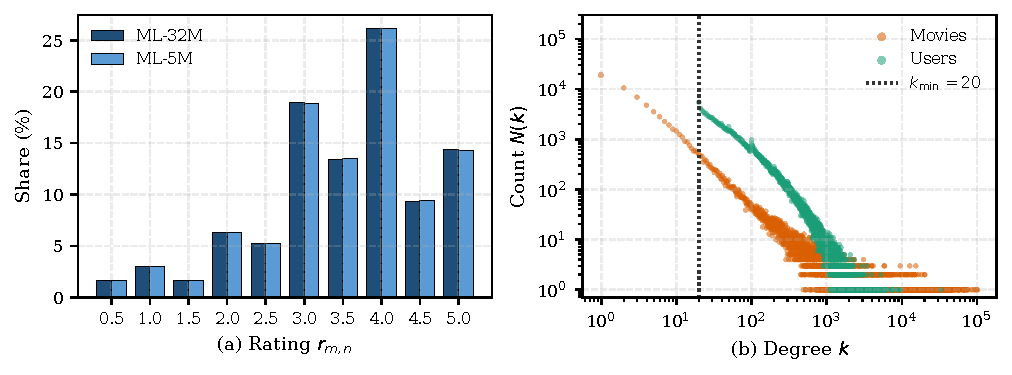
\includegraphics[width=\columnwidth]{figures/fig1_dataset_distributions.pdf}}
\caption{Exploratory plots of the MovieLens-32M and 5M datasets. \textbf{(a)} Percentage of ratings at each star value from $0.5$ to $5.0$, showing a peak at $4.0$ stars and lower counts on half-star values. \textbf{(b)} Log-log plot of the number of movies and users with $k$ ratings on MovieLens-32M, showing clear power-law tails and the minimum cutoff of $k_{\min}=20$ ratings per user.}
\label{fig:dataset_distributions}
\end{center}
\vskip -0.2in
\end{figure}

\cref{fig:dataset_distributions}(a) shows the distribution of star ratings from $0.5$ to $5.0$ on both MovieLens-32M and the 5M subset. The two datasets have almost identical rating proportions (within $0.02\%$ on every bar). Two simple patterns stand out:
\begin{enumerate}
    \item \textbf{Users Tend to Give High Ratings:} The average rating is $\mu = 3.540$ (with standard deviation $\sigma = 1.059$), which is well above the middle of the scale ($2.75$). The most common rating is $4.0$ stars ($26.15\%$ of all ratings, or $8{,}367{,}654$ ratings), followed by $3.0$ stars ($18.92\%$) and $5.0$ stars ($14.36\%$). Very low ratings ($0.5$, $1.0$, and $1.5$ stars combined) make up only $6.26\%$ of the data. This happens because people mostly choose to watch movies they expect to like \cite{koren2009matrix}.
    \item \textbf{Whole Stars Are Used More Than Half Stars:} Every half-star rating ($0.5, 1.5, 2.5, 3.5, 4.5$) appears much less often than the whole-star ratings next to it. For instance, $3.5$ stars is $13.41\%$ of the data, whereas $3.0$ is $18.92\%$ and $4.0$ is $26.15\%$. There are two reasons for this: MovieLens only added half-star ratings in 2003 (older ratings were whole numbers only), and many users naturally prefer round numbers when rating quickly.
\end{enumerate}

\cref{fig:dataset_distributions}(b) plots the degree distribution on a log-log scale: the horizontal axis is the number of ratings $k$, and the vertical axis is how many movies or users have exactly $k$ ratings. Both curves follow a straight line over several orders of magnitude on the log-log plot, which is the signature of a power law $P(k) \propto k^{-\alpha}$ \cite{clauset2009power}. However, movies and users behave very differently on the left side of the plot:
\begin{itemize}
    \item \textbf{Long Tail of Unpopular Movies:} Movie rating counts range from $k=1$ all the way to $k_{\max} = 102{,}929$ (\emph{The Shawshank Redemption (1994)}). Out of $84{,}432$ movies in MovieLens-32M, $16{,}895$ movies have only $1$ rating, and half of all movies have $5$ ratings or fewer (median $= 5.0$), even though the average movie has $379.0$ ratings. Using the standard maximum-likelihood formula for the power-law exponent \cite{clauset2009power} on the tail ($k_{\text{tail}} = 50$),
    \begin{equation}
        \hat{\alpha} = 1 + |\mathcal{T}| \left(\sum_{i \in \mathcal{T}} \ln \frac{k_i}{k_{\text{tail}} - 0.5}\right)^{-1},
        \label{eq:clauset_mle}
    \end{equation}
    gives a slope of $\hat{\alpha}_{\mathcal{I}} = 1.48$ for movies. A small group of blockbuster movies gets most of the ratings, while most of the catalog sits in the sparse long tail.
    \item \textbf{Sharp Cutoff at $k_{\min} = 20$ for Users:} Unlike movies, the user curve in \cref{fig:dataset_distributions}(b) stops suddenly at a vertical line at $k_{\min} = 20$ on MovieLens-32M (minimum $20$, median $73.0$, mean $159.2$, maximum $33{,}332$). This happens because the creators of the MovieLens dataset removed all users with fewer than $20$ ratings before releasing the data \cite{harper2015movielens}. Above $k = 20$, user activity follows a power law with slope $\hat{\alpha}_{\mathcal{U}} = 1.90$. Because of this rule, every user in the dataset has at least $20$ ratings (around $16$ in the training set), whereas thousands of movies have only $1$ or $2$ ratings. This makes cold-start much harder on the movie side than on the user side, which motivates our genre model in \cref{sec:genre_model}.
\end{itemize}

\section{Models and Optimization}
\label{sec:bias_model}

In this section, we present all three models developed in this paper and derive their Alternating Least Squares (ALS) optimization steps: (1) the baseline bias-only model, (2) the matrix factorization model with user and movie trait vectors $U$ and $V$, and (3) the genre-regularized matrix factorization model that incorporates movie genre metadata into the item prior, followed by our parallel in-place Cholesky implementation.

\subsection{Bias-Only Model}
\label{sec:bias_model_sub}

Before learning latent vectors, it is helpful to build a simple baseline model that captures general rating habits. Some users are generous and give high scores to almost everything ($a_m > 0$), while others are strict critics ($a_m < 0$). Likewise, popular classics get high scores from most viewers ($b_n > 0$), while weak movies get low scores ($b_n < 0$). The bias-only model predicts:
\begin{equation}
    \hat{r}_{m,n} = \mu + a_m + b_n,
    \label{eq:bias_model_pred}
\end{equation}
where $\mu$ is the average training rating ($\mu = 3.5404$ on MovieLens-32M), $a_m \in \mathbb{R}$ is the bias of user $m$, and $b_n \in \mathbb{R}$ is the bias of movie $n$.

\bibliography{references}
\bibliographystyle{icml2023}
\end{document}
